\documentclass[a4paper,twoside,12pt]{book}

\usepackage[usenames,dvipsnames]{xcolor}


%% === nezbytné balíčky:
\usepackage{lmodern}
% \usepackage[T1]{fontenc}    % kódování písma
%\usepackage[IL2]{fontenc}  % kódování písma

\usepackage[utf8]{inputenc}     % vstupní znaková sada tohoto dokumentu: UTF-8
%\usepackage[cp1250]{inputenc}  % vstupní znaková sada tohoto dokumentu: Windows 1250
%\usepackage[latin2]{inputenc}  % vstupní znaková sada tohoto dokumentu: ISO Latin 2

\usepackage[czech]{babel} % česky psaná práce, typografická pravidla. Překládejte pomocí "latex.exe" nebo "pdflatex.exe"
%\usepackage{czech} % česky psaná práce. Překládejte pomocí "pdfCSlatex.exe" ("cslatex.exe" asi bude mít problém s balíkem geometry)

\usepackage[a4paper, hmarginratio=3:2]{geometry} % využití A4 stránky a nastavení okrajů (u vazby bude širší)

\usepackage{pdfpages} % pokud nemáte formulář "Zadání bak./dipl. práce" naskenovaný jako PDF, tak ZAKOMENTUJTE
\usepackage[hidelinks]{hyperref} % v PDF budou klikací odkazy ("hidelinks" je nebude rámovat)

%% === balíčky, které se mohou hodit:
%\usepackage{encxvlna} % postará se o spojky a předložky, které dle českých pravidel nesmí být na konci řádku. Dokumentace: http://texdoc.net/texmf-dist/doc/generic/encxvlna/encxvlna.pdf (chová se správně k "vnitřku" listings?)

\usepackage{graphicx} % balíček pro vkládání rastrových grafických souborů (PNG apod.)
%\usepackage{epsfig} % balíčky pro vkládání grafických souborů typu EPS
% \usepackage{float} % rozšířené možnosti umístění obrázků
% \restylefloat{table}
\usepackage{pifont}

%\usepackage{caption} % pro popisky obrázků, tabulek atd.

\usepackage{tabularx} % rozšířené možnosti tabulek
\usepackage{longtable}

% \usepackage{tabu} % jiný balík pro rozšířené možnosti tabulek

\usepackage{listings}  % balíček vhodný pro ukázky zdrojového kódu v~textu práce/příloh. Nutno nastavit! http://ftp.cvut.cz/tex-archive/macros/latex/contrib/listings/listings.pdf
% \usepackage[autoload=true]{jlcode}
\usepackage{amsmath} % balíček pro pokročilou matematickou sazbu
\usepackage{amsfonts}
% \usepackage{color} % pro možnost barevného textu
%\usepackage{fancybox} % umožňuje pokročilé rámečkování
\usepackage{url}
\usepackage{bm}
\usepackage{hyperref}
\usepackage{threeparttable}
%\usepackage{index} % nutno použít v případě tvorby rejstříku balíčkem makeindex
%\newindex{default}{idx}{ind}{Rejstřík} % zavádí rejstřík v případě použití balíku index
\usepackage{csquotes}
\MakeOuterQuote{"}

\frenchspacing % za větou bude mezislovní mezera (v anglických textech je mezera za větou delší)
\widowpenalty=1000 % "síla" zákazu vdov (= jeden řádek ze začátku odstavce na konci stránky)
\clubpenalty=1000 % "síla" zákazu sirotků (= jeden řádek/slovo z konce odstavce samostatně na začátku stránky)
\brokenpenalty=1000 % "síla" zákazu zlomu stránky za řádkem, který má na konci rozdělené slovo

\topmargin=-15mm      % horní okraj trochu menší
\textwidth=150mm      % šířka textu na stránce
\textheight=240mm     % "výška" textu na stránce


\pagenumbering{arabic} % číslování stránek arabskými číslicemi
\pagestyle{plain}      % stránky číslované dole uprostřed

\parindent=0pt % odsazení 1. řádku odstavce
\parskip=7pt   % mezera mezi odstavci

%% --- zde jsou zavedeny některé "konstanty" - některé musíte změnit! --- %%
\newcommand{\cvut}{České vysoké učení technické v~Praze}
\newcommand{\fjfi}{Fakulta jaderná a fyzikálně inženýrská}
\newcommand{\ksi}{Katedra softwarového inženýrství}
\newcommand{\km}{Katedra matematiky}
\newcommand{\program}{Aplikace přírodních věd} % změňte, pokud máte jiný stud. program
\newcommand{\obor}{Aplikace informatiky v přírodních vědách} % změňte, pokud máte kurzívujiný obor

\newcommand{\druh}{Diplomová práce} % nebo "Diplomová práce"
\newcommand{\woman}{a} % pokud jste ŽENA, ZMĚŇTE na: ...{\woman}{a} (je to do Prohlášení)

\newcommand{\logoCVUT}{
\includegraphics{symbol_cvut_konturova_verze_cb.pdf}} % logo ČVUT -- podle grafického manuálu ČVUT platného od prosince 2016. Pokud nevyhovuje PDF-verze, tak použijte jinou variantu loga: https://www.cvut.cz/logo-a-graficky-manual -> "Symbol a logo ČVUT v Praze"). Pokud chcete logo úplně vynechat, zadejte místo "\includegraphics{...}" text "\vspace{35mm}"

% přesně podle formuláře "Zadání bak./dipl. práce" VYPLŇTE:
\newcommand{\nazevczT}{Analýza příčin vzniku shrinku produktů společnosti na základě logistických dat}    % český název práce (přesně podle zadání!)
\newcommand{\nazevenT}{Root Cause Analysis of Shrinkage Based on Logistics Data}          % anglický název práce (přesně podle zadání!)
\newcommand{\nazevcz}{Analýza příčin vzniku shrinku produktů společnosti na základě logistických dat}    % český název práce (přesně podle zadání!)
\newcommand{\nazeven}{Root Cause Analysis of Shrinkage Based on Logistics Data}          % anglický název práce (přesně podle zadání!)
\newcommand{\autor}{Bc. Anna Radová}   % vyplňte své jméno a příjmení (s akademickým titulem, máte-li jej)
\newcommand{\vedouci}{Ing. Martin Plajner, Ph.D.} % vyplňte jméno a příjmení vedoucího práce, včetně titulů, např.: Doc. Ing. Ivo Malý, Ph.D.
\newcommand{\pracovisteVed}{Oddělení matematické teorie rozhodování, Ústav teorie informace a automatizace AV ČR, v.v.i.} % ZMĚŇTE, pokud vedoucí Vaší práce není z KSI
\newcommand{\konzultant}{--} % POKUD MÁTE určeného konzultanta, NAPIŠTE jeho jméno a příjmení
\newcommand{\pracovisteKonz}{--} % POKUD MÁTE konzultanta, NAPIŠTE jeho pracoviště

% podle skutečnosti VYPLŇTE:
\newcommand{\rok}{2023}  % rok odevzdání práce (jen rok odevzdání, nikoli celý akademický rok!)
\newcommand{\kde}{Praze} % studenti z Děčína ZMĚNÍ na: "Děčíně" (doplní se k "prohlášení")

\newcommand{\klicova}{Datová analýza, Logistika}   % zde NAPIŠTE česky max. 5 klíčových slov
\newcommand{\keyword}{Data Analysis, Logistics}       % zde NAPIŠTE anglicky max. 5 klíčových slov (přeložte z češtiny)
\newcommand{\abstrCZ}{}

% zde NAPIŠTE abstrakt v češtině (cca 7 vět, min. 80 slov)
\newcommand{\abstrEN}{} % zde NAPIŠTE abstrakt v angličtině

\newcommand{\prohlaseni}{Prohlašuji, že jsem svou bakalářskou práci vypracoval\woman{} samostatně a použil\woman{} jsem pouze podklady (literaturu, projekty, SW atd.) uvedené v přiloženém seznamu.} % text prohlášení můžete mírně upravit :-)

\newcommand{\podekovani}{Chtěla bych poděkovat doktoru Ing. Martinu Plajnerovi, Ph.D. za vedení mé diplomové práce, za cenné rady, připomínky a trpělivost během tvorby této práce a za čas strávený touto pomocí. Dále děkuji své rodině a manželovi za obrovkou podporu při psaní práce a během celého studia.} % NAPIŠTE poděkování, např. svému vedoucímu:
% Děkuji Ing. Eleonoře Krtečkové, Ph.D. za vedení mé bakalářské práce a za podnětné návrhy, které ji obohatily.
% NEBO:
% Děkuji vedoucímu práce doc. Pafnutijovi Snědldítětikaši, Ph.D. za neocenitelné rady a pomoc při tvorbě bakalářské práce.

\newcommand{\ti}{\textit} % zkrácený příkaz pro kurzívu
\newcommand{\tb}{\textbf} % zkrácený příkaz pro tučné písmo
\newcommand{\tn}{\texttt} % zkrácený příkaz pro neproporcionalni písmo


% Vzhled kódu
\renewcommand{\lstlistingname}{Kód}
%New colors defined below
\definecolor{julia}{rgb}{0.12,0.6,0.08}
\definecolor{julia}{rgb}{0.12,0.6,0.08}
\definecolor{chromeyellow}{rgb}{1.0, 0.65, 0.0}
\definecolor{byzantine}{rgb}{0.74, 0.2, 0.64}
\definecolor{airforceblue}{rgb}{0.36, 0.54, 0.66}
\definecolor{backcolor}{rgb}{0.95,0.95,0.95}
\definecolor{border}{rgb}{0.98,0.98,0.98}

% Takhle se pouziva pro ukazky kodu
% \begin{lstlisting}[caption=Definice metody size pro dataset Iris, label=Kod:ImSiz]
%     size(::Iris) = (150, 0, 0)
% \end{lstlisting}

% napise julia> barevne
\newcommand{\jul}{\textcolor{julia}{julia> }}


\newenvironment{repl}
{\fontfamily{cmvtt}\selectfont \begin{mdframed}

}{\end{mdframed}}

\usepackage[linewidth=1pt]{mdframed}


\newcolumntype{L}{>{\centering\arraybackslash}m{2cm}}
\newcolumntype{N}{>{\centering\arraybackslash}m{1.7cm}}
\newcolumntype{M}{>{\centering\arraybackslash}m{1.6cm}}
\newcolumntype{K}{>{\centering\arraybackslash}m{1.5cm}}
\newcolumntype{S}{>{\centering\arraybackslash}m{1cm}}
\renewcommand{\arraystretch}{1.3}

\newcommand{\cmark}{\textcolor{green!80!black}{\ding{51}}}
\newcommand{\xmark}{\textcolor{red}{\ding{55}}}




% Listing style
\lstdefinelanguage{julia}
{%
%
% julia's keywords:
%
morekeywords=[1]
{%
abstract type,baremodule,begin,break,catch,ccall,const,continue,do,else,elseif,%
end,export,finally,for,function,global,if,import,in,isa,let,local,macro,module,%
mutable struct,primitive type,quote,return,struct,try,using,where,while, function%
},%
%
% julia's literals:
%
morekeywords=[2]
{%
ARCH,ARGS,Apr,April,Aug,August,BINDIR,CPU_NAME,CPU_THREADS,C_NULL,DEPOT_PATH,%
DL_LOAD_PATH,Dec,December,ENDIAN_BOM,ENV,Feb,February,Fri,Friday,I,%
ISODateFormat,ISODateTimeFormat,ISOTimeFormat,Inf,Inf16,Inf32,Inf64,%
InsertionSort,JIT,Jan,January,Jul,July,Jun,June,KERNEL,LOAD_PATH,MACHINE,Mar,%
March,May,MergeSort,Mon,Monday,NaN,NaN16,NaN32,NaN64,Nov,November,Oct,October,%
PROGRAM_FILE,QuickSort,RFC1123Format,RTLD_DEEPBIND,RTLD_FIRST,RTLD_GLOBAL,%
RTLD_LAZY,RTLD_LOCAL,RTLD_NODELETE,RTLD_NOLOAD,RTLD_NOW,RoundDown,%
RoundFromZero,RoundNearest,RoundNearestTiesAway,RoundNearestTiesUp,RoundToZero,%
RoundUp,STDLIB,Sat,Saturday,Sep,September,Sun,Sunday,Thu,Thursday,Tue,Tuesday,%
VERSION,WORD_SIZE,Wed,Wednesday,catalan,devnull,dlext,e,eulergamma,false,%
golden,im,missing,nothing,pi,stderr,stdin,stdout,true,undef,γ,π,φ,ℯ%
},%
%
% julia's built-ins:
%
morekeywords=[3]
{%
AbstractArray,AbstractChannel,AbstractChar,AbstractDict,AbstractDisplay,%
AbstractFloat,AbstractIrrational,AbstractLogger,AbstractMatrix,AbstractREPL,%
AbstractRNG,AbstractRange,AbstractSerializer,AbstractSet,AbstractSparseArray,%
AbstractSparseMatrix,AbstractSparseVector,AbstractString,AbstractUnitRange,%
AbstractVecOrMat,AbstractVector,AbstractWorkerPool,Adjoint,Any,ArgumentError,%
Array,AssertionError,Atomic,Base64DecodePipe,Base64EncodePipe,BasicREPL,%
Bidiagonal,BigFloat,BigInt,BitArray,BitMatrix,BitSet,BitVector,Bool,%
BoundsError,BroadcastStyle,BunchKaufman,CachingPool,CapturedException,%
CartesianIndex,CartesianIndices,Cchar,Cdouble,Cfloat,Channel,Char,Cholesky,%
CholeskyPivoted,Cint,Cintmax_t,Clong,Clonglong,ClusterManager,Cmd,CodeInfo,%
CodeInstance,Colon,Complex,ComplexF16,ComplexF32,ComplexF64,CompositeException,%
Condition,ConsoleLogger,Cptrdiff_t,Cshort,Csize_t,Cssize_t,Cstring,Cuchar,%
Cuint,Cuintmax_t,Culong,Culonglong,Cushort,Cvoid,Cwchar_t,Cwstring,DataType,%
Date,DateFormat,DatePeriod,DateTime,Day,DenseArray,DenseMatrix,DenseVecOrMat,%
DenseVector,Diagonal,Dict,DimensionMismatch,Dims,DivideError,DomainError,%
EOFError,Eigen,Enum,ErrorException,Event,Exception,ExponentialBackOff,Expr,%
FDWatcher,FILE,Factorization,FileMonitor,Float16,Float32,Float64,FolderMonitor,%
Function,Future,GeneralizedEigen,GeneralizedSVD,GeneralizedSchur,GenericArray,%
GenericDict,GenericOrder,GenericSet,GenericString,GitConfig,GitRepo,GlobalRef,%
GotoNode,HMAC_CTX,HTML,Hermitian,Hessenberg,Hour,IO,IOBuffer,IOContext,%
IOStream,IPAddr,IPv4,IPv6,IdDict,IndexCartesian,IndexLinear,IndexStyle,%
InexactError,InitError,Int,Int128,Int16,Int32,Int64,Int8,Integer,%
InterruptException,InvalidStateException,Irrational,KeyError,LAPACKException,%
LDLt,LQ,LU,LinRange,LineEditREPL,LineInfoNode,LineNumberNode,LinearIndices,%
LoadError,LogLevel,LowerTriangular,MIME,Matrix,MersenneTwister,Method,%
MethodError,MethodInstance,Microsecond,Millisecond,Minute,Missing,%
MissingException,Module,Month,NTuple,NamedTuple,Nanosecond,NewvarNode,Nothing,%
NullLogger,Number,OrdinalRange,OutOfMemoryError,OverflowError,Pair,%
PartialQuickSort,Period,PermutedDimsArray,PhiCNode,PhiNode,PiNode,Pipe,%
PollingFileWatcher,PosDefException,ProcessExitedException,%
ProcessFailedException,Ptr,QR,QRPivoted,QuoteNode,RandomDevice,%
RankDeficientException,Rational,RawFD,ReadOnlyMemoryError,Real,ReentrantLock,%
Ref,Regex,RegexMatch,RemoteChannel,RemoteException,RoundingMode,SHA1_CTX,%
SHA224_CTX,SHA256_CTX,SHA2_224_CTX,SHA2_256_CTX,SHA2_384_CTX,SHA2_512_CTX,%
SHA384_CTX,SHA3_224_CTX,SHA3_256_CTX,SHA3_384_CTX,SHA3_512_CTX,SHA512_CTX,%
SSAValue,SVD,Schur,Second,SegmentationFault,Serializer,Set,SharedArray,%
SharedMatrix,SharedVector,Signed,SimpleLogger,SingularException,Slot,%
SlotNumber,Some,SparseMatrixCSC,SparseVector,SpinLock,StackFrame,%
StackOverflowError,StackTrace,StepRange,StepRangeLen,StreamREPL,StridedArray,%
StridedMatrix,StridedVecOrMat,StridedVector,String,StringIndexError,SubArray,%
SubString,SubstitutionString,SymTridiagonal,Symbol,Symmetric,SystemError,%
TCPSocket,Task,TaskFailedException,TestSetException,Text,TextDisplay,Time,%
TimePeriod,TimeType,TimeZone,Timer,TmStruct,Transpose,Tridiagonal,Tuple,%
TypeError,TypeVar,TypedSlot,UDPSocket,UInt,UInt128,UInt16,UInt32,UInt64,UInt8,%
UTC,UUID,UndefInitializer,UndefKeywordError,UndefRefError,UndefVarError,%
UniformScaling,Union,UnionAll,UnitLowerTriangular,UnitRange,%
UnitUpperTriangular,Unsigned,UpperHessenberg,UpperTriangular,UpsilonNode,Val,%
Vararg,VecElement,VecOrMat,Vector,VersionNumber,WeakKeyDict,WeakRef,Week,%
WorkerConfig,WorkerPool,Year,ZeroPivotException,%
DatasetName,Tabular,Split, GrayImage, MLImage,Image, Classification, Regression,%
Iris, Adult, MNIST, Nuclear, Gisette, Labels, Ionosphere, Train, L2, Boston 
},%
%
% julia's macros:
%
morekeywords=[4]
{%
@MIME_str,@NamedTuple,@__DIR__,@__FILE__,@__LINE__,@__MODULE__,@__dot__,%
@allocated,@assert,@async,@b_str,@big_str,@boundscheck,@ccall,@cfunction,@cmd,%
@code_llvm,@code_lowered,@code_native,@code_typed,@code_warntype,%
@dateformat_str,@debug,@deprecate,@distributed,@doc,@doc_str,@dump,@edit,%
@elapsed,@enum,@error,@eval,@evalpoly,@everywhere,@fastmath,@fetch,@fetchfrom,%
@functionloc,@generated,@gensym,@goto,@html_str,@inbounds,@inferred,@info,%
@inline,@int128_str,@ip_str,@isdefined,@label,@less,@logmsg,@macroexpand,%
@macroexpand1,@md_str,@noinline,@nospecialize,@polly,@printf,@profile,@r_str,%
@raw_str,@s_str,@show,@simd,@spawn,@spawnat,@specialize,@sprintf,@static,@sync,%
@task,@test,@test_broken,@test_deprecated,@test_logs,@test_nowarn,@test_skip,%
@test_throws,@test_warn,@testset,@text_str,@threadcall,@threads,@time,@timed,%
@timev,@uint128_str,@v_str,@var,@view,@views,@warn,@which%
},%
%
% julia's functions:
%
morekeywords=[5]
{%
BLAS,Base,Base64,Broadcast,CRC32c,Compiler,Core,Dates,DelimitedFiles,%
Distributed,Docs,FileWatching,FormatMessage,GC,GetLastError,IR,%
InteractiveUtils,Intrinsics,Iterators,LAPACK,LibGit2,Libc,Libdl,LinearAlgebra,%
Logging,Main,Markdown,MathConstants,Meta,Mmap,PipeBuffer,Printf,Profile,REPL,%
Random,SHA,Serialization,SharedArrays,Sockets,SparseArrays,StackTraces,%
SuiteSparse,Sys,Test,Threads,UUIDs,Unicode,__precompile__,abs,abs2,abs_float,%
abspath,accept,accumulate,accumulate!,acos,acosd,acosh,acot,acotd,acoth,acsc,%
acscd,acsch,add_float,add_float_fast,add_int,add_ptr,addprocs,adjoint,adjoint!,%
adjust,all,all!,allunique,and_int,angle,any,any!,append!,applicable,apropos,%
argmax,argmin,arraylen,ascii,asec,asecd,asech,ashr_int,asin,asind,asinh,%
asyncmap,asyncmap!,atan,atand,atanh,atexit,atomic_add!,atomic_and!,atomic_cas!,%
atomic_fence,atomic_max!,atomic_min!,atomic_nand!,atomic_or!,atomic_sub!,%
atomic_xchg!,atomic_xor!,atreplinit,axes,axpby!,axpy!,backtrace,base64decode,%
base64encode,basename,big,bind,binomial,bitcast,bitrand,bitreverse,bitrotate,%
bitstring,blockdiag,broadcast,broadcast!,broadcast_axes,%
broadcast_preserving_zero_d,broadcastable,bswap,bswap_int,bunchkaufman,%
bunchkaufman!,bytes2hex,bytesavailable,calloc,canonicalize,cat,catch_backtrace,%
cbrt,cd,ceil,ceil_llvm,cglobal,channel_from_id,check_same_host,checkbounds,%
checked_sadd_int,checked_sdiv_int,checked_smul_int,checked_srem_int,%
checked_ssub_int,checked_uadd_int,checked_udiv_int,checked_umul_int,%
checked_urem_int,checked_usub_int,checkindex,chmod,cholesky,cholesky!,chomp,%
chop,chown,circcopy!,circshift,circshift!,cis,clamp,clamp!,cld,clear!,%
clipboard,close,cluster_cookie,cmp,coalesce,code_llvm,code_lowered,code_native,%
code_typed,code_warntype,codepoint,codeunit,codeunits,collect,complex,cond,%
condskeel,conj,conj!,connect,contains,convert,copy,copy!,copy_transpose!,%
copysign,copysign_float,copyto!,cos,cosc,cosd,cosh,cospi,cot,cotd,coth,count,%
count!,count_ones,count_zeros,countfrom,countlines,cp,cpu_info,cpu_summary,%
crc32c,cross,csc,cscd,csch,ctime,ctlz_int,ctpop_int,cttz_int,cumprod,cumprod!,%
cumsum,cumsum!,current_logger,current_task,cycle,datetime2julian,datetime2rata,%
datetime2unix,day,dayabbr,dayname,dayofmonth,dayofquarter,dayofweek,%
dayofweekofmonth,dayofyear,daysinmonth,daysinyear,daysofweekinmonth,deepcopy,%
default_worker_pool,deg2rad,delete!,deleteat!,denominator,deserialize,det,%
detach,detect_ambiguities,detect_unbound_args,diag,diagind,diagm,diff,digest!,%
digits,digits!,dirname,disable_logging,disable_sigint,display,displayable,%
displaysize,div,div_float,div_float_fast,divrem,dlclose,dllist,dlopen,dlopen_e,%
dlpath,dlsym,dlsym_e,doc,dot,dotview,download,drop,dropdims,droptol!,dropwhile,%
dropzeros,dropzeros!,dump,eachcol,eachindex,eachline,eachmatch,eachrow,%
eachslice,edit,eigen,eigen!,eigmax,eigmin,eigvals,eigvals!,eigvecs,eltype,%
empty,empty!,endswith,enumerate,eof,eps,eq_float,eq_float_fast,eq_int,errno,%
error,esc,escape_string,eval,evalfile,evalpoly,exit,exp,exp10,exp2,expanduser,%
expm1,exponent,extrema,factorial,factorize,falses,fd,fdio,fetch,fieldcount,%
fieldname,fieldnames,fieldoffset,fieldtype,fieldtypes,filemode,filesize,fill,%
fill!,filter,filter!,finalize,finalizer,find_library,findall,findfirst,%
findlast,findmax,findmax!,findmin,findmin!,findnext,findnz,findprev,first,%
firstdayofmonth,firstdayofquarter,firstdayofweek,firstdayofyear,firstindex,%
flatten,fld,fld1,fldmod,fldmod1,flipsign,flipsign_int,float,floatmax,floatmin,%
floor,floor_llvm,flush,flush_cstdio,fma,fma_float,foldl,foldr,foreach,fpext,%
fpiseq,fpislt,fptosi,fptoui,fptrunc,free,free_memory,frexp,fullname,%
functionloc,gcd,gcdx,gensym,get,get!,get_zero_subnormals,getaddrinfo,%
getalladdrinfo,getfield,gethostname,getindex,getipaddr,getipaddrs,getkey,%
getnameinfo,getpeername,getpid,getproperty,getsockname,givens,global_logger,%
gperm,graphemes,hasfield,hash,haskey,hasmethod,hasproperty,hcat,hessenberg,%
hessenberg!,hex2bytes,hex2bytes!,hmac_sha1,hmac_sha224,hmac_sha256,%
hmac_sha2_224,hmac_sha2_256,hmac_sha2_384,hmac_sha2_512,hmac_sha384,%
hmac_sha3_224,hmac_sha3_256,hmac_sha3_384,hmac_sha3_512,hmac_sha512,homedir,%
hour,html,htol,hton,hvcat,hypot,identity,ifelse,ignorestatus,imag,in,%
include_dependency,include_string,indexin,indexpids,init_worker,insert!,%
instances,interrupt,intersect,intersect!,inv,invmod,invoke,invperm,invpermute!,%
isa,isabspath,isabstracttype,isapple,isapprox,isascii,isassigned,isbits,%
isbitstype,isblockdev,isbsd,ischardev,iscntrl,isconcretetype,isconst,isdefined,%
isdiag,isdigit,isdir,isdirpath,isdisjoint,isdispatchtuple,isdragonfly,isempty,%
isequal,iseven,isexecutable,isexpr,isfifo,isfile,isfinite,isfreebsd,%
ishermitian,isimmutable,isinf,isinteger,isinteractive,isjsvm,isleapyear,isless,%
isletter,islink,islinklocaladdr,islinux,islocked,islowercase,ismarked,%
ismissing,ismount,ismutable,isnan,isnetbsd,isnothing,isnumeric,isodd,isone,%
isopen,isopenbsd,ispath,isperm,isposdef,isposdef!,ispow2,isprimitivetype,%
isprint,ispunct,isqrt,isreadable,isreadonly,isready,isreal,issetequal,issetgid,%
issetuid,issocket,issorted,isspace,issparse,issticky,isstructtype,issubnormal,%
issubset,issuccess,issymmetric,istaskdone,istaskfailed,istaskstarted,%
istextmime,istril,istriu,isunix,isuppercase,isvalid,iswindows,iswritable,%
isxdigit,iszero,iterate,join,join_multicast_group,joinpath,julian2datetime,%
keys,keytype,kill,kron,last,lastdayofmonth,lastdayofquarter,lastdayofweek,%
lastdayofyear,lastindex,latex,launch,lcm,ldexp,ldiv!,ldlt,ldlt!,le_float,%
le_float_fast,leading_ones,leading_zeros,leave_multicast_group,length,%
less,listen,listenany,llvmcall,lmul!,loadavg,localindices,lock,log,log10,log1p,%
log2,logabsdet,logdet,lowercase,lowercasefirst,lowrankdowndate,%
lowrankdowndate!,lowrankupdate,lowrankupdate!,lpad,lq,lq!,lshr_int,lstat,%
lstrip,lt_float,lt_float_fast,ltoh,lu,lu!,lyap,macroexpand,malloc,manage,map,%
map!,mapfoldl,mapfoldr,mapreduce,mapslices,mark,match,max,maximum,maximum!,%
maxintfloat,merge,merge!,mergewith,mergewith!,methods,methodswith,microsecond,%
millisecond,min,minimum,minimum!,minmax,minute,mkdir,mkpath,mktemp,mktempdir,%
mod,mod1,mod2pi,modf,month,monthabbr,monthday,monthname,mtime,mul!,mul_float,%
mul_float_fast,mul_int,muladd,muladd_float,mv,myid,nameof,names,nanosecond,%
ncodeunits,ndigits,ndims,ne_float,ne_float_fast,ne_int,neg_float,%
neg_float_fast,neg_int,nextfloat,nextind,nextpow,nextprod,nfields,nnz,%
nonmissingtype,nonzeros,norm,normalize,normalize!,normpath,not_int,notify,now,%
nprocs,nthreads,ntoh,ntuple,nullspace,numerator,nworkers,nzrange,objectid,%
occursin,oftype,one,ones,oneunit,only,open,operm,opnorm,or_int,ordschur,%
ordschur!,pairs,parent,parentindices,parentmodule,parse,partialsort,%
partialsort!,partialsortperm,partialsortperm!,partition,pathof,peakflops,peek,%
permute,permute!,permutedims,permutedims!,pinv,pipeline,pkgdir,pmap,pointer,%
pointer_from_objref,pointerref,pointerset,poll_fd,poll_file,pop!,popat!,%
popdisplay,popfirst!,position,powermod,precision,precompile,prepend!,prevfloat,%
prevind,prevpow,print,println,printstyled,process_exited,process_messages,%
process_running,procs,prod,prod!,product,promote,promote_rule,promote_shape,%
promote_type,propertynames,push!,pushdisplay,pushfirst!,put!,pwd,qr,qr!,%
quarterofyear,quot,rad2deg,rand,rand!,randcycle,randcycle!,randexp,randexp!,%
randn,randn!,randperm,randperm!,randstring,randsubseq,randsubseq!,range,rank,%
rata2datetime,rationalize,rdiv!,read,read!,readavailable,readbytes!,readchomp,%
readdir,readdlm,readline,readlines,readlink,readuntil,real,realloc,realpath,%
recv,recvfrom,redirect_stderr,redirect_stdin,redirect_stdout,redisplay,reduce,%
reenable_sigint,reflect!,reim,reinterpret,relpath,rem,rem2pi,rem_float,%
rem_float_fast,remote,remote_do,remotecall,remotecall_fetch,remotecall_wait,%
remoteref_id,repeat,repeated,replace,replace!,repr,reset,reshape,resize!,rest,%
rethrow,retry,reverse,reverse!,reverseind,rint_llvm,rm,rmprocs,rmul!,rot180,%
rotate!,rotl90,rotr90,round,rounding,rowvals,rpad,rsplit,rstrip,run,schedule,%
schur,schur!,sdata,sdiv_int,searchsorted,searchsortedfirst,searchsortedlast,%
sec,secd,sech,second,seek,seekend,seekstart,selectdim,send,serialize,%
set_zero_subnormals,setdiff,setdiff!,setenv,setfield!,setindex!,setprecision,%
setproperty!,setrounding,sext_int,sha1,sha224,sha256,sha2_224,sha2_256,%
sha2_384,sha2_512,sha384,sha3_224,sha3_256,sha3_384,sha3_512,sha512,shl_int,%
show,show_sexpr,showable,showerror,shuffle,shuffle!,sign,signbit,signed,%
significand,similar,sin,sinc,sincos,sincosd,sind,sinh,sinpi,sitofp,size,%
sizehint!,sizeof,skip,skipchars,skipmissing,sle_int,sleep,slt_int,something,%
sort,sort!,sortperm,sortperm!,sotrtslices,sparse,sparsevec,spdiagm,splice!,%
split,splitdir,splitdrive,splitext,splitpath,sprand,sprandn,sprint,spzeros,%
sqrt,sqrt_llvm,sqrt_llvm_fast,srem_int,stacktrace,start_worker,srtartswith,%
stat,step,strerror,strftime,stride,strides,string,stringmime,strip,strptime,%
sub_float,sub_float_fast,sub_int,sub_ptr,subtypes,success,sum,sum!,summary,%
supertype,supertypesd,svd,svd!,svdvals,svdvals!,sylvester,symdiff,symdiff!,%
symlink,systemerror,systemsleep,take,take!,takewhile,tan,tand,tanh,%
task_local_storage,tempdir,tempname,textwidth,thisind,threadhid,throw,time,%
time_ns,timedwait,titlecase,to_indices,today,tofirst,tolast,tonext,toprev,%
total_memory,touch,tr,trailing_ones,trailing_zeros,transcode,transpose,%
transpose!,tril,tril!,ttriu,triu!,trues,trunc,trunc_int,trunc_llvm,truncate,%
trylock,tryparse,tuple,typeassert,typeintersect,typejoin,typemax,typemin,%
typeof,udiv_int,uitofp,ule_int,ult_int,unescape_string,uunion,union!,unique,%
unique!,unix2datetime,unlock,unmark,unsafe_copyto!,unsafe_load,%
unsafe_pointer_to_objref,unsafe_read,unsafe_store!,unsafe_string,unsafe_trunc,%
unsafe_wrap,unsafe_wsrite,unsigned,unwatch_folder,update!,uperm,uppercase,%
uppercasefirst,uptime,urem_int,uuid1,uuid4,uuid5,uuid_version,valtype,values,%
varinfo,vcat,vec,versioninfo,view,wait,walkdir,watcah_file,watch_folder,week,%
which,widemul,widen,with,with_logger,withenv,worker_id_from_socket,workers,%
write,writedlm,xor,xor_int,year,yearmonth,yearmonthday,yield,yieldto,zero,%
zeros,ziext_int,zip, load, name, prep, preprocess, url, checksum,%
target, headers, problem, message, postprocess, getdata, split_traintest,%
split_trainvalidtest, meanstd, binarize, info
},%
%
%
sensitive=true,%
%
alsoother={$},%$%
alsodigit={_},%
%
morecomment=[l]{\#},%
morecomment=[n]{\#=}{=\#},%
%
morestring=[b]{"},%
% just activate the next command if you dont use ' as the transposition
% operator! comment out line 1283 in that case, too!
%morestring=[m]{'},%
morestring=[s]{"""}{"""},%
morestring=[s]{L"}{"},%
morestring=[s]{MIME"}{"},%
morestring=[s]{b"}{"},%
morestring=[s]{big"}{"},%
morestring=[s]{dateformat"}{"},%
morestring=[s]{doc"}{"},%
morestring=[s]{html"}{"},%
morestring=[s]{int128"}{"},%
morestring=[s]{ip"}{"},%
morestring=[s]{md"}{"},%
morestring=[s]{pkg"}{"},%
morestring=[s]{r"}{"},%
morestring=[s]{raw"}{"},%
morestring=[s]{s"}{"},%
morestring=[s]{text"}{"},%
morestring=[s]{uint128"}{"},%
morestring=[s]{v"}{"},%
morestring=[s]{var"}{"},%
%
}[keywords,comments,strings]

\definecolor{jlbase}{RGB}{68, 68, 68}       % julia's base color
\definecolor{jlkeyword}{RGB}{230, 9, 72}    % julia's keywords
\definecolor{jlliteral}{RGB}{11, 195, 212}  % julia's literals
\definecolor{jlbuiltin}{RGB}{7, 94, 235}    % julia's built-ins
\definecolor{jlmacros}{RGB}{255, 166, 0}    % julia's macros
\definecolor{jlfunctions}{RGB}{11, 156, 25} % julia's functions
\definecolor{jlcomment}{RGB}{136, 136, 136} % julia's comments
\definecolor{jlstrnum}{RGB}{255, 166, 0}    % julia's strings or numbers
\definecolor{jlop}{RGB}{68, 68, 68}         % julia's operators

\lstdefinestyle{juliastyle}{
    captionpos = b,
    basicstyle=\ttfamily\footnotesize, 
    tabsize = 2,
    lineskip = -1.5pt,
    extendedchars = true,
    breaklines = true,
    upquote = true,
    tabsize = 4,
    aboveskip = {0.5\baselineskip},
    belowskip = {0.5\baselineskip},
    rulecolor=\color{Black},
    frame = shadowbox,
    rulesepcolor = \color{white!50!gray},
    columns = fixed,
    linewidth = \textwidth,
    xleftmargin = {0.05\textwidth},
    xrightmargin = {0.05\textwidth},
    keywordstyle={[1]\color{jlkeyword}\bfseries},
    keywordstyle={[2]\color{jlliteral}},
    keywordstyle={[3]\color{jlbuiltin}},
    keywordstyle={[4]\color{jlmacros}},
    keywordstyle={[5]\color{jlfunctions}},
    commentstyle={\color{jlcomment}},
    stringstyle={\color{jlstrnum}},
    identifierstyle={\color{jlbase}},
    showstringspaces=false,
}
\lstset{style = juliastyle, language = julia}


\lstdefinelanguage{juliarepl}
{%
% Purple
morekeywords=[1]{
    DatasetName, using%
},%
% Light blue
morekeywords=[2]{},%
% Blue
morekeywords=[3]{
    Image, Tabular, v1.6, pkg, add
},
% Yellow
morekeywords=[4]{
    CIFAR10, CIFAR100, SVHN2, FashionMNIST, MNIST,
},
% Green
morekeywords=[5]{
    julia,
    ColorImage, GrayImage, Abalone, Adult, Boston, Carevaluation, Forestfires,
    Gisette, Ionosphere, Iris, Nuclear, Wine,
    listdatasets, info,
},
}[keywords]

\lstdefinelanguage{juliarepl2}
{%
% Purple
morekeywords=[1]{
    using
},%
% Light blue
morekeywords=[2]{Info},%
% Blue
morekeywords=[3]{
    Vector, Bool, Int64, DataFrame, String, Float64, Matrix, Any
},
% Yellow
morekeywords=[4]{
    Abalone, Adult, Carevaluation, Gisette, Ionosphere, Iris, Wine, FashionMNIST, MNIST, CIFAR10, CIFAR100, SVHN2, help,
},
% Green
morekeywords=[5]{
    julia, listdatasets, info, load, first, getheader, meanstd, normalize, binarize, collect
},
}[keywords]


% todo notes
\usepackage[colorinlistoftodos]{todonotes}

\begin{document}
%%%%%%%%%%%% TITULNÍ STRANA -- na následujících cca 30 řádků NESAHEJTE!!!  Generuje se AUTOMATICKY %%%%%%%%%%%%
\thispagestyle{empty}

\begin{center}
	{\LARGE
		\cvut\par
		\fjfi
	}
    \vspace{10mm}

    \begin{tabular}{c}
		\tb{\ksi} \\[3pt]
		\tb{Obor: \obor}\\
    \end{tabular}

   \vspace{10mm} \logoCVUT \vspace{15mm}

   {\huge \tb{\nazevczT}\par}
   \vspace{5mm}
   {\huge \tb{\nazevenT}\par}

   \vspace{15mm}
   {\Large \MakeUppercase{\druh}}

   \vfill
   {\large
    \begin{tabular}{ll}
    Vypracoval: & \autor\\
    Vedoucí práce: & \vedouci\\
    Rok: & \rok
    \end{tabular}
   }
\end{center}

\clearpage{\pagestyle{empty}\cleardoublepage} % prázdná stránka za tou "titulní", bez čísla

%%%%%%%%%%%% ZADÁNÍ PRÁCE %%%%%%%%%%%%
% Zadání (podepsané děkanem!) musíte NASKENOVAT. Ideálně jako 2stránkové PDF (soubor "zadani_cele.pdf").
% Před svázáním to v jednom výtisku VYMĚNÍTE ZA ORIGINÁLNÍ ZADÁNÍ (podepsané děkanem fakulty)!
\newpage  % SEM NESAHEJTE!
\thispagestyle{empty} % SEM NESAHEJTE!

%% zde podle toho, jak jste zadání naskenovali, VYBERTE variantu A, B nebo C:
%
% --- varianta A: zadání naskenované jako 2stránkové PDF:
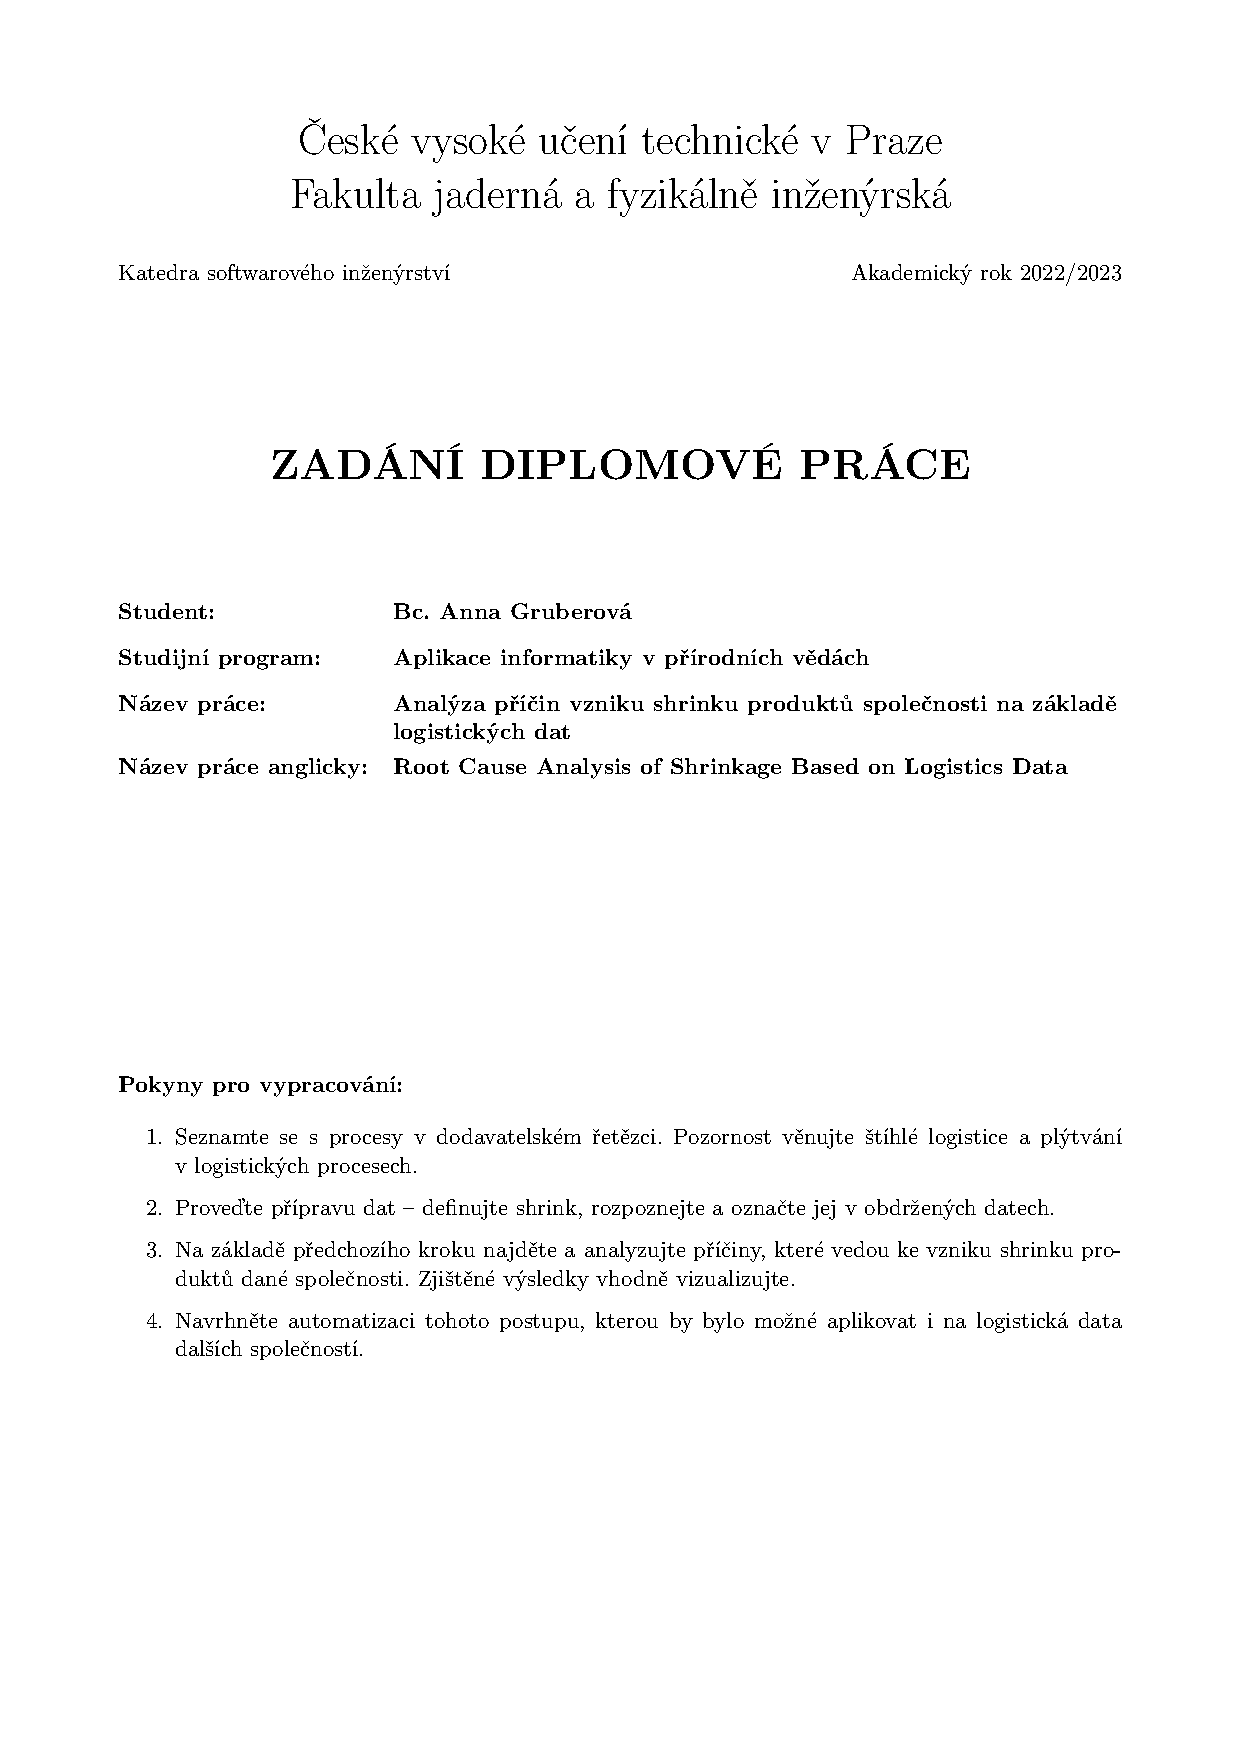
\includepdf[pages={1,2}]{zadaniDP.pdf} % NAHRAĎTE správným souborem!!!!DOPLNIT
%
%% --- varianta B: zadání naskenované jako jednotlivé stránky:
%\includepdf[pages={1}]{zadani1.pdf} % 1. strana zadání v PDF
%\includepdf[pages={1}]{zadani2.pdf} % 2. strana zadání v PDF
%
%% --- varianta C: zadání naskenované jako 2 samostatné obrázky:
%% 1. strana zadání
%\begin{center}
%     \includegraphics[width=1\textwidth]{zadani1.jpg}
%\end{center}
%% 2. strana zadání
%\newpage  % SEM NESAHEJTE!
%\thispagestyle{empty} % SEM NESAHEJTE!
%\begin{center}
%     \includegraphics[width=1\textwidth]{zadani2.jpg}zada
%\end{center}


%%%%%%%%%%%% Prohlášení -- SEM NESAHEJTE! Generuje se automaticky z výše nastavených maker \kde{} a \prohlaseni{}. %%%%%%%%%%%%
\newpage % SEM NESAHEJTE!
\thispagestyle{empty}  % SEM NESAHEJTE!

~ % SEM NESAHEJTE!
\vfill % prázdné místo. SEM NESAHEJTE!

\tb{Prohlášení} % SEM NESAHEJTE!

\vspace{1em} % vertikální mezera. SEM NESAHEJTE!
\prohlaseni

\vspace{2em}  % SEM NESAHEJTE!
\hspace{-0.5em}\begin{tabularx}{\textwidth}{X c}  % SEM NESAHEJTE!
V \kde\ dne .................... &........................................ \\	% SEM NESAHEJTE!
	& \autor
\end{tabularx}	% SEM NESAHEJTE!


%%%%%%%%%%%% Poděkování  %%%%%%%%%%%%
\newpage
\thispagestyle{empty}

~
\vfill % prázdné místo


% -- následující kus kódu (do "%%%%%%%%%%%% ABSTRAKT") můžete odstranit, pokud nechcete psát poděkování:
\tb{Poděkování}

\vspace{1em} % vertikální mezera
\podekovani
\begin{flushright}
\autor
\end{flushright}  % <------- tady končí stránka s poděkováním


%%%%%%%%%%%% ABSTRAKT atp. Je generován AUTOMATICKY podle maker nastavených na začátku souboru) %%%%%%%%%%%%
\newpage   % SEM NESAHEJTE!
\thispagestyle{empty}   % SEM NESAHEJTE!

% příprava:    (na následujících 8 řádků NESAHEJTE!)
\newbox\odstavecbox
\newlength\vyskaodstavce
\newcommand\odstavec[2]{%
    \setbox\odstavecbox=\hbox{%
         \parbox[t]{#1}{#2\vrule width 0pt depth 4pt}}%
    \global\vyskaodstavce=\dp\odstavecbox
    \box\odstavecbox}
\newcommand{\delka}{115mm} % šířka textů ve 2. sloupci tabulky

% použití přípravy:    % dovnitř "tabular" vůbec NESAHEJTE!
\begin{tabular}{ll}
  {\em Název práce:} & ~ \\
  \multicolumn{2}{l}{\bf \nazevcz} \\[1em]
  {\em Autor:} & \autor \\[1em]
  {\em Studijní program:} & \program \\
  {\em Obor:} & \obor \\
  {\em Druh práce:} & \druh \\[1em]
  {\em Vedoucí práce:} & \odstavec{\delka}{\vedouci\\ \pracovisteVed} \\
  {\em Konzultant:} & -- %\odstavec{\delka}{\konzultant \\ \pracovisteKonz}  % VYMAŽTE text "-- %" v případě, že jste neměli konzultanta
 \\[1em]
  \multicolumn{2}{l}{\odstavec{\textwidth}{{\em Abstrakt:} ~ \abstrCZ  }} \\[1em]
  {\em Klíčová slova:} & \odstavec{\delka}{\klicova} \\[2em]

  {\em Title:} & ~\\
  \multicolumn{2}{l}{\bf \nazeven}\\[1em]
  {\em Author:} & \autor \\[1em]
  \multicolumn{2}{l}{\odstavec{\textwidth}{{\em Abstract:} ~ \abstrEN  }} \\[1em]
  {\em Key words:} & \odstavec{\delka}{\keyword}
\end{tabular}



%%%%%%%%%%%% Obsah práce ... je generován AUTOMATICKY %%%%%%%%%%%%
\newpage  % SEM NESAHEJTE!
\parskip=0pt
\tableofcontents % SEM NESAHEJTE!
\parskip=7pt
\newpage % SEM NESAHEJTE!


%--------------------------------------------------------
%|         Zde začíná SAMOTNÁ PRÁCE (text)              |
%--------------------------------------------------------

\chapter*{Úvod} % SEM NESAHEJTE!
\addcontentsline{toc}{chapter}{Úvod} % SEM NESAHEJTE!
%
% %
% Tato diplomová práce se zabývá analýzou dat vybrané společnosti. Cílem práce je prozkoumat obdržená data, která se týkají tzv. shrinků. Jedná se o záznamy o produktech, které z~různých důvodů nemohly být prodány a kvůli tomu společnost přišla o zisk a vynaložila zbytečné náklady související s~nákupem a logistikou dotčených produktů. 

Na základě analýzy je třeba vyslovit hypotézy, které mohou souviset s~příčinou vzniku shrinku. Tyto hypotézy je třeba otestovat na datech a navrhnout tak možný postup pro hledání příčin existence shrinku produktů i v~datech dalších společností. 

% TODO

První kapitola se věnuje definici odborným pojmům z~logistiky, a to především z~odvětví, které se zabývá plýtváním. Popsány jsou tři hlavní typy plýtvání, dále jsou představeny možné zdroje plýtvání v~logistických procesech.

V následující kapitole se nachází teoretický popis metod, které jsem použila pro datovou analýzu. Jedná se o metody pro selekci příznaků a metodu GUHA. Dále jsou v~kapitole popsány důležité pojmy týkající se korelační analýzy. Závěr kapitoly je věnován popisu použitých nástrojů.

Ve třetí kapitole je definován pojem shrink a jeho klasifikace v~literatuře a v~obdrže-\\ných datech vybrané společnosti.

Další, čtvrtá kapitola popisuje způsob získání dat vybrané společnosti. Následuje popis jednotlivých databázových tabulek a jejich sloupců. Zbylá část kapitoly se zabývá přípravou vzorku pro další analýzy. Tedy kterou částí dat se zabývat na základě četnosti a metod pro selekci proměnných. Prozkoumány jsou vztahy mezi jednotlivými příznaky.

V páte kapitole je popsán business intelligence report vytvořený v~ aplikaci Power BI, který vizualizuje obdržená data. První část obsahuje popis jednotlivých stránek interaktivního reportu a popis použitých vizuálů. Druhá část je věnována závěrům, které z~reportu vyplývají.

Šestá kapitola obsahuje návrh řešení pro kategorizaci shrinkovaných produktů pomocí korelační analýzy. V~kapitole je uveden postup analýzy a popis implementace v~jazyce Python. Konec kapitoly je věnován ukázce výsledků této metody.

Poslední kapitola analyzuje data pomocí procedury GUHA a metody 4ftMiner. V~této kapitole bylo vysloveno několik hypotéz a následně byla ověřována jejich platnost.



% - Data
%     - jak jsou data uložená v~DB u zákazníka
%         - provázané
%     - SQL příkazy
%     - výběr proměnných
%     - target hodnoty - cost, množství
%     - produktová Hierarchie
% - Vymazaní outlierů
%     - outlier metody
%     - businessově

% - Co vysvetluje target
%     - Miner
%     - PCA

% - Korelační analýza mezi produkty v~rámci kategorie
%     - korelace 
% - Rozčlenění produktů

% - Vizualizace dat
%     - Jak funguje PBI
%     - Seznam metri
Tato diplomová práce se zabývá analýzou dat vybrané společnosti. Cílem práce je prozkoumat obdržená data, která se týkají tzv. shrinků. Jedná se o záznamy o produktech, které z~různých důvodů nemohly být prodány a kvůli tomu společnost přišla o zisk a vynaložila zbytečné náklady související s~nákupem a logistikou dotčených produktů. 

Na základě analýzy je třeba vyslovit hypotézy, které mohou souviset s~příčinou vzniku shrinku. Tyto hypotézy je třeba otestovat na datech a navrhnout tak možný postup pro hledání příčin existence shrinku produktů i v~datech dalších společností. 

% TODO

První kapitola se věnuje definici odborným pojmům z~logistiky, a to především z~odvětví, které se zabývá plýtváním. Popsány jsou tři hlavní typy plýtvání, dále jsou představeny možné zdroje plýtvání v~logistických procesech.

V následující kapitole se nachází teoretický popis metod, které jsem použila pro datovou analýzu. Jedná se o metody pro selekci příznaků a metodu GUHA. Dále jsou v~kapitole popsány důležité pojmy týkající se korelační analýzy. Závěr kapitoly je věnován popisu použitých nástrojů.

Ve třetí kapitole je definován pojem shrink a jeho klasifikace v~literatuře a v~obdrže-\\ných datech vybrané společnosti.

Další, čtvrtá kapitola popisuje způsob získání dat vybrané společnosti. Následuje popis jednotlivých databázových tabulek a jejich sloupců. Zbylá část kapitoly se zabývá přípravou vzorku pro další analýzy. Tedy kterou částí dat se zabývat na základě četnosti a metod pro selekci proměnných. Prozkoumány jsou vztahy mezi jednotlivými příznaky.

V páte kapitole je popsán business intelligence report vytvořený v~ aplikaci Power BI, který vizualizuje obdržená data. První část obsahuje popis jednotlivých stránek interaktivního reportu a popis použitých vizuálů. Druhá část je věnována závěrům, které z~reportu vyplývají.

Šestá kapitola obsahuje návrh řešení pro kategorizaci shrinkovaných produktů pomocí korelační analýzy. V~kapitole je uveden postup analýzy a popis implementace v~jazyce Python. Konec kapitoly je věnován ukázce výsledků této metody.

Poslední kapitola analyzuje data pomocí procedury GUHA a metody 4ftMiner. V~této kapitole bylo vysloveno několik hypotéz a následně byla ověřována jejich platnost.



% - Data
%     - jak jsou data uložená v~DB u zákazníka
%         - provázané
%     - SQL příkazy
%     - výběr proměnných
%     - target hodnoty - cost, množství
%     - produktová Hierarchie
% - Vymazaní outlierů
%     - outlier metody
%     - businessově

% - Co vysvetluje target
%     - Miner
%     - PCA

% - Korelační analýza mezi produkty v~rámci kategorie
%     - korelace 
% - Rozčlenění produktů

% - Vizualizace dat
%     - Jak funguje PBI
%     - Seznam metri

\chapter{}

\cite{bib:Jones}

\section{Logistika}

\subsection*{Definice Logistiky}

Logistika zahrnuje všechny operace, které se týkají doručení zboží nebo služeb od výrobce k zákazníkovi, s výjimkou samotné výroby zboží nebo provádění služby. Výrobou je naopak rozuměno vše, co mění podobu materiálu.
Během výroby se však logistika uplatňuje, například jako přesun materiálu nebo polotovarů mezi jednotlivými výrobními zařízeními. 
% Obdobně při poskytování služby je podstatné se zabývat 
Operace lze rozdělit do tří hlavních toků: materiálový, informační a finanční tok. Materiálový obsahuje všechny pohyby týkající se fyzického materiálu, tedy jeho získávání, přesuny a skladování, a to jak mezi zákazníky, dodavateli či výrobními areály a sklady, tak i vnitřní pohyby mezi produkčními linkami nebo skladovými pozicemi. Informační tok popisuje procesy vznikající během materiálového toku, dále se do něj řadí analýzy již proběhlých toků a plánování a předpovědi budoucích toků. Poslední kategorie, finanční tok mapuje náklady způsobené předešlými dvěma zmíněnými toky.\cite{bib:Baudin}

Pojem logistika je úzce propojen s pojmem Supply Chain Management (SCM)\footnote{Do češtiny lze Supply Chain Management přeložit jako řízení či správa dodavatelského řetězce. V českém prostředí se používá jak anglická tak česká podoba.}. Zatímco logistika se zabývá toky zboží, služeb či lidí, Supply Chain Management zahrnuje operace logistiky, navíc ale sleduje vztahy mezi procesory, které koordinuje a optimalizuje za účelem naplnění určitých cílů. Tímto cílem bývá často snížení nákladů v rámci částí procesu nebo zvýšení konkurenceschopnosti podniku \cite{bib:IIMudaipur}. Supply Chain Management se tedy prolíná s pojmem logistika a bývají často zaměňovány. Důvodem může být i to, že se jedná o nový pojem, který byl poprvé použitý v roce 1982.\cite{bib:Christopher} 

\section{Štíhlá logistika}

Rozdělení 

\subsection*{MUDA}
\subsection*{MULA}

\chapter*{Závěr} % SEM NESAHEJTE!
\addcontentsline{toc}{chapter}{Závěr} % SEM NESAHEJTE!
%
Cílem práce bylo nalézt možné příčiny vzniku shirnků produktu pro vybranou společnost a dále vytvořit prototyp řešení pro aplikování dané analýzy na data dalších společností.

V teoretické části práce jsem se seznámila s~odbornými pojmy z~odvětví logistiky a druhy plýtvání v~tomto oboru. Dále jsem sepsala princip hlavních použitých metod pro výběr proměnných a metody GUHA. Dále jsem definovala používané odborné pojmy týkající se analýzy. Teorie se také věnuje popisu nástrojů, které jsem použila při analýze. Především se jedná o popis aplikace Power BI pro vytváření interaktivních business intelligence reportů.

Samostatná kapitola se zabývá pojmem shrink. Je uvedena jeho definice a nastíněna problematika tohoto pojmu. Pak jsem popsala konkrétní typy evidovaných shrinků dané společnosti.

Nejprve jsem se seznámila s~obdrženými daty. Z rozsáhlého množství záznamů jsem vybrala vzorový měsíc s~nižším počtem záznamů, na kterém jsem prováděla všechny analýzy. Vzhledem k~velkému počtu záznamů a především vzhledem k~sezónnosti produktů a proměnlivé poptávky trhu během roku nebylo vhodné provádět analýzu na všech dostupných datech nebo na celém roku. Z databáze a externích zdrojů jsem vytipovala další data, která by pomohla vysvětlit existenci shrinků.

Stažená surová data jsem sjednotila pro další práci do samostatného datasetu. Vznikl tak dataset s~mnoha příznaky, který bylo třeba dále očistit. Odstranila jsem outliery a vybrala pouze ten typ shrinku, jehož hodnota ztracených nákladů činila nejvíce. Obdobně jsem postupovala i co se týče kategorií produktů, kterých se shrinky týkají. Z businessové stránky problému je jasné, že ke shrinku může čas od času dojít a je třeba se soustředit pouze na ty produkty, u kterých k~němu dochází opakovaně. 
Prozkoumala jsem jednotlivé příznaky datasetu a označila ty, které jsou na sobě závislé a které naopak mohou pomoci vysvětlit shrink. 

Data jsem analyzovala pomocí interaktivního reportu. Odhaleny tak byly kategorie, kterých se shrink nejvíce týká. Nejvíce postižené jsou čerstvé výrobky. Došlo také k~porovnání evidovaných shrinků mezi jednotlivými prodejnami a regiony. Ukázalo se, že umístění prodejny nemá podle dat významný vliv na vznik shrinku. 

% Na základě těchto zjištění byly stanoveny hypotézy o souvislostech vedoucích ke vzniku shrinků. Pomocí různých metod byly tyto hypotézy potvrzeny nebo vyvráceny pro konkrétní produkty.

Provedla jsem korelační analýzu, která zkoumá závislosti mezi datasetem se shrinky a tržbami. Jedná se jak o tržby shrinkovaného produktu, tak promoční tržby ostatních produktů v~kategorii definované úrovně produktové hierarchie. Korelační analýza takto dokáže rozdělit shrinkované produkty do několika kategorií v~závislosti na hodnotě korelačního koeficientu. Zde je důležité upozornit, že kauzalita vysvětlená korelací byla businessovým rozhodnutím. V~případě pochybení by následky pro společnost nebyly fatální. Naopak se jedná o postup, který společnost může snadno ovlivnit.   Společnost totiž může plánovat své promoakce s~ohledem na kategorizaci produktů. 
Korelační analýzu jsem spustila na obdržených datech a diskutovala jsem výsledky pro nejčastěji shrinkované kategorie  

V návaznosti na tuto práci by mohlo být dále otestováno celé portfolio vybrané společnosti.
Navržený způsob rozdělení produktů do kategorií podle jejich vztahu k~ostatním produktům by mohl být převeden do soběstačného nástroje, který nevyžaduje programátorský přístup a může tak být využitý například při navrhování promoakcí produktů. Tomu samozřejmě musí předcházet několikanásobné testování na datech z~více zdrojů, které ale nebyly k~dispozici pro tuto diplomovou práci.

% Bylo vyhodnoceno, kterou částí rozsáhlých dat se zabývat na základě četnosti a metod pro selekci proměnných. Prozkoumány jsou vztahy mezi jednotlivými příznaky.




%%%%%%%%%%%% SEZNAM POUŽITÝCH ZDROJŮ (LITERATURA) %%%%%%%%%%%%
\clearpage  % SEM NESAHEJTE!
\addcontentsline{toc}{chapter}{Literatura} % SEM NESAHEJTE!


	% formát: ČSN ISO 690. Můžete si to vygenerovat na http://www.citacepro.com (přihlaste se přes odkaz "ČVUT"), umí to vygenerovat TeX
	% řazení: abecedně podle autora (resp. prvního slova, není-li znám autor)

	% \bibitem{odkaz} Autor. \ti{Název knihy}. Město. Nakladatelství. Rok. 
    % \bibitem{bib:ai}


\begin{thebibliography}{1}

\bibitem{bib:Baudin}
BAUDIN, Michel. \textit{Lean Logistics: The Nuts and Bolts of Delivering Materials and Goods}. New York: Productivity Press, 2005. ISBN 978-1563272967.

\bibitem{bib:Christopher}
CHRISTOPHER, Martin. \textit{Logistics \& Supply Chain Management}. 5th ed. Harlow: Pearson Education Limited, 2016. ISBN 9781292083797.
% https://books.google.cz/books?id=NIfQCwAAQBAJ&printsec=frontcover&dq=Logistics+and+Supply+Chain+Management&hl=cs&sa=X&redir_esc=y#v=onepage&q=Logistics%20and%20Supply%20Chain%20Management&f=false

\bibitem{bib:literatura}
HASTIE, T., TIBSHIRANI R., FRIEDMAN J. H. \textit{The elements of statistical learning: data
mining, inference, and prediction.} 2nd ed. New York: Springer, 2009. Springer series in statistics. ISBN 978-0-387-84857-0.

\bibitem{bib:IIMudaipur}
What is the difference between Logistics and Supply Chain Management. In: \textit{IIM Udaipur Chronicles} [online]. 11. 10. 2019. [cit. 2022-11-07] Dostupné z: \url{https://www.iimu.ac.in/blog/what-is-the-difference-between-logistics-and-supply-chain-management/}

\bibitem{bib:Jirsak}
JIRSÁK, Petr, MERVART, Michal, VINŠ, Marek. \textit{Logistika pro ekonomy -- vstupní logistika.} 1. vydání. Praha: Wolters Kluwer ČR, 2012.

\bibitem{bib:Jones}
JONES, Daniel T., HINES Peter  a RICH Nick. Lean logistics. \textit{International Journal of Physical Distribution \& Logistics Management}. 1997, \textbf{27}(3/4), 153-173. ISSN 0960-0035. Dostupné z: doi:10.1108/09600039710170557

\bibitem{bib:PCA1}
KURITA, Takio. \textit{Principal component analysis (PCA). Computer Vision: A Reference Guide}. 2019, 1-4. [cit. 2022-11-07] Dostupné z: \url{https://link.springer.com/content/pdf/10.1007/978-3-030-03243-2\_649-1.pdf}

\bibitem{bib:PCA2}
TONHAUSEROVÁ, Zuzana. \textit{Metoda hlavních komponent a její aplikace}. Diplomová práce. Olomouc: UPOL. 2013 [cit. 2023-12-18]. Dostupné z: \url{https://theses.cz/id/iwan2b/Zuzana_Tonhauserov_-_Metoda_hlavnch_komponent.txt}

\bibitem{bib:PCA3}
JAADI, Zakaria. \textit{A Step-by-Step Explanation of Principal Component Analysis (PCA)
} [online].  [cit. 2023-03-04]. Dostupné z: \url{https://builtin.com/data-science/step-step-explanation-principal-component-analysis}


\bibitem{bib:thiel}
MILLS, Peter. \textit{Efficient statistical classification of satellite measurements}. In: \textit{International Journal of Remote Sensing.Informa UK Limited}, 2011, 32(21): 6109–6132. [cit. 2023-12-18]. Dostupné z: doi:10.1080/01431161.2010.507795

\bibitem{bib:multi}
ZAMAZAL, Petr. \textit{Statistická analýza rozsáhlých dat z průmyslu}. Diplomová práce, vedoucí Šomplák, Radovan. Vysoké účení technické v Brně, 2010.

\bibitem{bib:MCA1}
DI FRANCO, Giovanni. \textit{Multiple correspondence analysis: one only or several techniques?}. Quality \& Quantity, 2016, 50.3: 1299-1315. [cit. 2023-03-05]. Dostupné z: doi:10.1007/s11135-015-0206-0

\bibitem{bib:MCA2}
ABDI, Hervé, VALENTIN, Dominique. \textit{Multiple correspondence analysis}. In: \textit{Encyclopedia of measurement and statistics}. 2007, 2.4: 651-657. [cit. 2023-03-05]. Dostupné z: \url{https://personal.utdallas.edu/\~Herve/Abdi-MCA2007-pretty.pdf}

\bibitem{bib:MI}
NAVARA, Mirko. \textit{Teorie informace.} [online). 3. 1. 2017 [cit. 2023-12-15]. Dostupné z: \url{https://cmp.felk.cvut.cz/~navara/psi/TI_ebook.pdf}

\bibitem{bib:MI2}
PŘICHYSTAL, Jan. \textit{Úvod do teorie informace.} [online). 3. 1. 2007 [cit. 2023-12-15]. Dostupné z: \url{https://akela.mendelu.cz/~jprich/predn/teoinf.pdf}

\bibitem{bib:MI3}
KROUPA, Tomáš. \textit{Úvod do teorie informace: Matematické základy komprese a digitální komunikace.} [online). [cit. 2023-12-15]. Dostupné z: \url{https://math.fel.cvut.cz/en/people/gollova/tik/TI_prednasky.pdf}

\bibitem{bib:CA1}
GREENACRE, Michael. \textit{Correspondence analysis in practice}. chapman and hall/crc, 2017. [cit. 2023-03-05]. 

\bibitem{bib:CA2}
Correspondence analysis. In \textit{Wikiwand} [online]. [cit. 2023-03-06]. Dostupné z: \url{https://www.wikiwand.com/en/Correspondence\_analysis}

\bibitem{bib:Wronka}
WRONKA, Anna. LEAN LOGISTICS. \textit{Journal of Positive Management}. 2017, \textbf{7}(2), 55-63. ISSN 2392-1412. Dostupné z: doi:10.12775/JPM.2016.012

\bibitem{bib:seven}
SUTHERLAND Joel, BENNETT Bob. \textit{The Seven Deadly Wastes of Logistics: Applying Toyota Production System Principles to Create Logistics Value}. Bethelem, PA: Lehigh University, 2007. Dostupné z: \url{https://www.researchgate.net/publication/265356600}

\bibitem{bib:LW1}
SKHMOT, Nawras. \textit{The Lean Way Blog: The 8 Wastes of Lean. The Lean Way} [online]. 5. 8. 2017 [cit. 2022-11-17]. Dostupné z: \url{https://theleanway.net/The-8-Wastes-of-Lean}

\bibitem{bib:LW2}
SKHMOT, Nawras. \textit{The Lean Way Blog: What is Lean?. The Lean Way} [online]. 5. 8. 2017 [cit. 2022-11-17]. Dostupné z: \url{https://theleanway.net/what-is-lean}

\bibitem{bib:LW3}
SKHMOT, Nawras. \textit{The Lean Way Blog: What is Muda, Mura, and Muri?. The Lean Way} [online]. 5. 8. 2017 [cit. 2022-11-17]. Dostupné z:
 \url{https://theleanway.net/muda-mura-muri}

\bibitem{bib:DefShrink}
Learning the Lingo: 3 definitions related to unsold food inventory. In: \textit{Blog - Spoiler Alert} [online]. 17. 06. 2019. [cit. 2022-02-07] Dostupné z: \url{https://blog.spoileralert.com/3-definitions-unsold-food-inventory}

\bibitem{prince}
HALFORD, M. Prince., \textit{Prince} [online]. [cit. 2023-03-08]. Dostupné z: \url{https://github.com/MaxHalford/prince}

\bibitem{bib:encoding}
BAIJAYANTA, Roy., \textit{All about Categorical Variable Encoding } [online]. [cit. 2023-03-13]. Dostupné z: \url{https://towardsdatascience.com/all-about-categorical-variable-encoding-305f3361fd02}

\bibitem{bib:scikit}
scikit-learn Machine Learning in Python [online]. 2023 [cit. 2023-03-21]. Dostupné z: \url{https://scikit-learn.org/stable/}

\bibitem{bib:scikit-multiclass}
Multiclass and multioutput algorithms. scikit [online]. [cit. 2023-04-10]. Dostupné z: \url{https://scikit-learn.org/stable/modules/multiclass.html} 

\bibitem{bib:statology}
BOBBITT, Zach. \textit{How to Interpret Cramer's V} In \textit{Statology} [online]. 2021 [cit. 2023-03-21]. Dostupné z: \url{https://www.statology.org/interpret-cramers-v/}

\bibitem{bib:correl}
ZYCHLINSKI, Shaked. \textit{The Search for Categorical Correlation} [online]. 2018 [cit. 2023-03-14]. Dostupné z: \url{https://towardsdatascience.com/the-search-for-categorical-correlation-a1cf7f1888c9}

\bibitem{bib:MB}
HOLČÍK, Jiří, KOMENDA, Martin (eds.) a kol. \textit{Matematická biologie: e-learningová učebnice} [online]. 
1. vydání. Brno: Masarykova univerzita, 2015. [cit. 2023-03-14]. ISBN 978-80-210-8095-9.

\bibitem{bib:chooseregression}
FROST, Jim. \textit{Choosing the correct type of regression analysis.} [online]. [cit. 2023-04-10]. Dostupné z: \url{https://statisticsbyjim.com/regression/choosing-regression-analysis/}

\bibitem{bib:multiregression}
Multiclass logistic regression. In \textit{Refactored} [online]. [cit. 2023-04-10]. Dostupné z: \url{https://refactored.ai/}

\bibitem{bib:rf}
BIAU, Gérard; SCORNET, Erwan. \textit{A random forest guided tour}. In: \textit{Test} [online]. 2016, 25: 197-227. [cit. 2023-04-10].

\bibitem{bib:rfgb}
LOK, Leon. \textit{Decision trees, random forests and gradient boosting: What's the difference?} [online]. 5. 1. 2022. [cit. 2023-04-10]. Dostupné z: \url{https://leonlok.co.uk/blog/decision-trees-random-forests-gradient-boosting-whats-the-difference/}

\bibitem{bib:scipyPearson}
Scipy.stats.pearsonr. In \textit{scipy.stats.pearsonr - SciPy v1.11.4 Manual} [online]. [cit. 2023-12-10]. Dostupné z: \url{https://docs.scipy.org/doc/scipy/reference/generated/scipy.stats.pearsonr.html} 

\bibitem{bib:czso}
BILÍK, Jan. \textit{Databáze demografických údajů za vybraná města ČR} [online]. 30. 05. 2023 [cit. 2023-07-12]. Dostupné z: \url{https://www.czso.cz/csu/czso/databaze-demografickych-udaju-za-vybrana-mesta-cr}


\bibitem{bib:shrink1}
HUBER, Nicholas, MICHAEL, Katina, \textit{Minimizing Product Shrinkage across the Supply Chain using Radio Frequency Identification: a Case Study on a Major Australian Retailer,}. In: \textit{International Conference on the Management of Mobile Business (ICMB 2007)}. Toronto, ON, Canada, 2007, 45-45. [cit. 2023-12-16]. Dostupné z: doi: 10.1109/ICMB.2007.43.

\bibitem{bib:shrink2}
BECK, Adrian. \textit{Moving beyond shrinkage: developing a definition and typology of total retail loss.} 2018, 93–110. https://doi.org/10.1057/s41284-017-0090-5

\bibitem{bib:GUHA}
RAUCH, Jan, ŠIMŮNEK, Milan \textit{Metoda GUHA a Systém LISp-Miner} [online]. [cit. 2023-12-15]. Dostupné z: \url{lispminer.vse.cz}

\bibitem{bib:GUHAclever}
MASA, Petr. \textit{CleverMiner -- Beyond apriori.} [online]. [cit. 2023-12-15]. Dostupné z: \url{www.cleverminer.org}

\bibitem{bib:correlation}
de WINTER, Joost, GOSLING, Samuel, POTTER, Jeff. \textit{Comparing the Pearson and Spearman Correlation Coefficients Across Distributions and Sample Sizes: A Tutorial Using Simulations and Empirical Data. Psychological Methods.} 2016, 21: 273-290. Dostupné z: doi: 10.1037/met0000079. 

\end{thebibliography}
	
% 
	
	
% \bibliographystyle{unsrt}
% \bibliography{tex/bibliofrafie}


%%%%%%%%%%%% PŘÍLOHY PRÁCE %%%%%%%%%%%%
\newpage % SEM NESAHEJTE!
\addcontentsline{toc}{chapter}{Přílohy} % SEM NESAHEJTE!
\appendix % SEM NESAHEJTE!


%%%%%%%%%%%% Příloha A (tj. 1. kapitola v rámci příloh) %%%%%%%%%%%%

\chapter{Obsah přiloženého CD}
%
BP\_Gruberova.pdf -- soubor s elektronickou verzí této bakalářské práce.

PreprocessData -- složka se zdrojovými kódy naimplementovaného balíku \newline PreprocessData.jl.

%
% \input{priloha_A.tex} % text vkládán ze souboru, kde je i příkaz \chapter{...}


\end{document} % SEM NESAHEJTE! Konec.
